% This document is used for Daya Bay MACRO PMT pressure test report


\documentclass{beamer}
\usepackage{graphicx}

%\setlength{\unitlength}{\textwidth}

\setbeamertemplate{navigation symbols}{}
\setbeamertemplate{footline}[page number]
\setbeamertemplate{caption}[numbered]
%\setbeamerfont{purisa}
\usetheme{default}
\logo{
\includegraphics[height=1cm]{Dyb_logo.png}}
\begin{document}
\title{Status of MACRO PMT pressure tests at SAB}
\author{Logan Lebanowski, Shih-Kai Lin}
\institute{University of Houston}
\date{Sep 23, 2010}

\begin{frame}
\begin{center}
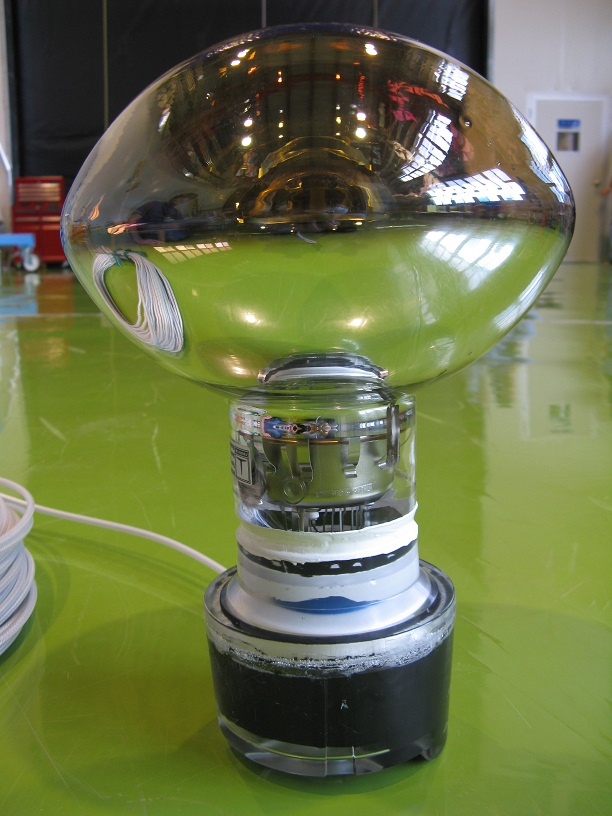
\includegraphics[height=4cm]{IMG_1048.jpg}
\end{center}
\titlepage
\end{frame}


\begin{frame}{pressure test results}
\begin{itemize}
	\item As of September 23, we have passed 47 of 50 PMTs.
	\item 11 PMTs were tested during the past week (September 16 - September 22). PMT 8870
	had a hole in the cable jacket. It was fixed and tested again.
\end{itemize}
\begin{table}
\small
\begin{tabular}{c|c|c|c|c}
%\setlength{\tabcolsep}{2pt}
	SN & mass (g) & pressure (psig) & test time (h:m) & result \\
	\hline
	7851 & 564 & 12.1 & 14:48 & PASS$^1$ \\
	7127 & 582 & 12.2 & 8:51 & PASS$^2$ \\
	7820 & 595.5 & 12.0 & 14:44 & PASS$^3$ \\
	7267 & 643.5 & 12.0 & 8:44 & PASS$^2$ \\
	7934 & 609 & 12.0 & 14:48 & FAIL$^4$ \\
	8430 & 554 & 12.0 & 47:23 & FAIL$^5$ \\
	8870 & 587.5 & 12.0 & 7:27 & PASS$^2$ \\
	7899 & 566 & 12.0 & 16:24 & PASS$^3$ \\
	7765 & 573 & 12.1 & 7:05 & PASS$^3$ \\
	7471 & 601 & 12.0 & 14:56 & PASS$^1$ \\
	%6873 & 601.5 & 12.2 & 
\end{tabular}
\caption {pressure test result: For PASS/FAIL reasons, please see the table in the next slide.}
\end{table}
%\begin{itemize}
%	\item For PASS/FAIL reasons, please see the table in the next slide.
%\end{itemize}
\end{frame}

\begin{frame}{PASS/FAIL reasons}
	\setlength{\tabcolsep}{2pt}
	\small
	\begin{table}
		\begin{tabular}{|c|p{3.5in}|}
		\hline
		\textbf{number} & \textbf{reason} \\
		\hline
		\hline
		1 & Cable dry. No leaks or cracks. \\
		\hline
		2 & 1+Some water penetrated the mastic tape seal of the cable strain relief plug,
			but did not penetrate the UW cable plug. \\
		\hline
		3 & Moisture on the SHV end in the sealing tube. Conductivity test performed. \\
		\hline
		4 & Acrylic cap contains much water.(see photo) \\
		\hline
		5 & A big crack and a little hole in the PMT. Photocathode was gone.(see photo) \\
		\hline
		\end{tabular}
	\caption{PASS/FAIL reasons}
	\end{table}
\end{frame}

\begin{frame}{photos: PMT 7934}
%\framebox{
	%\begin{picture}(1.5,1.1)
	%	\put(100,-80){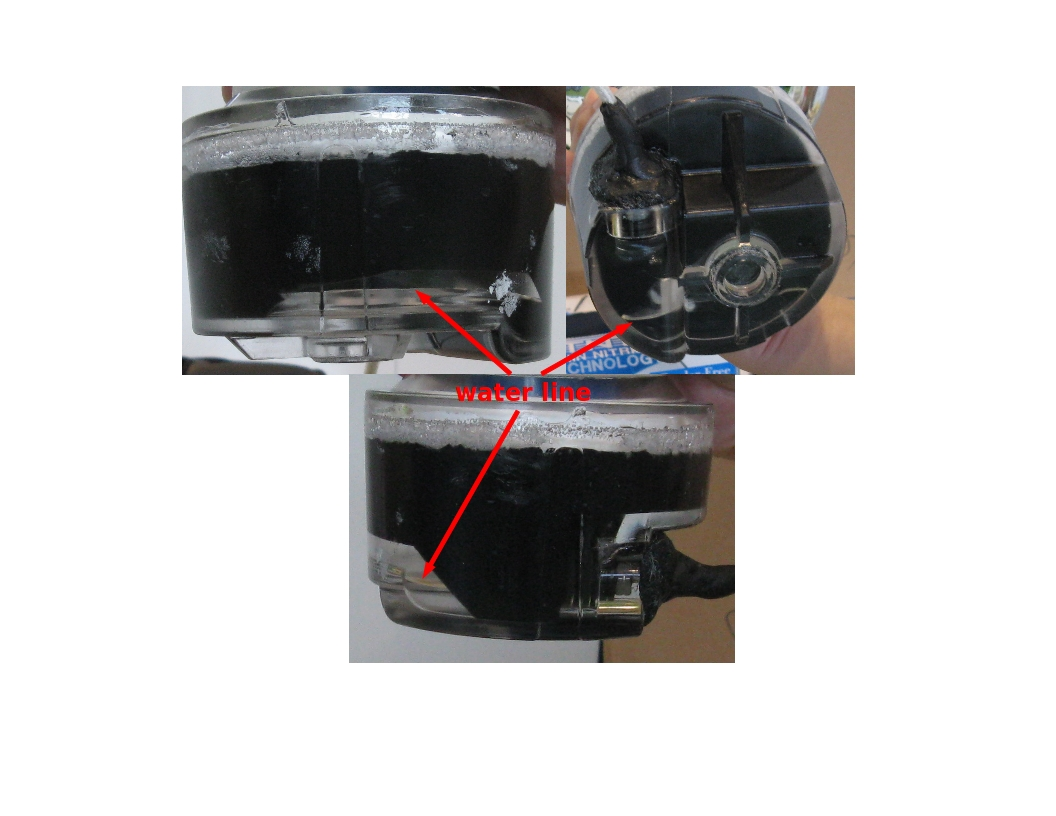
\includegraphics[width=30cm]{PMT7934.jpg}}
	%\end{picture}
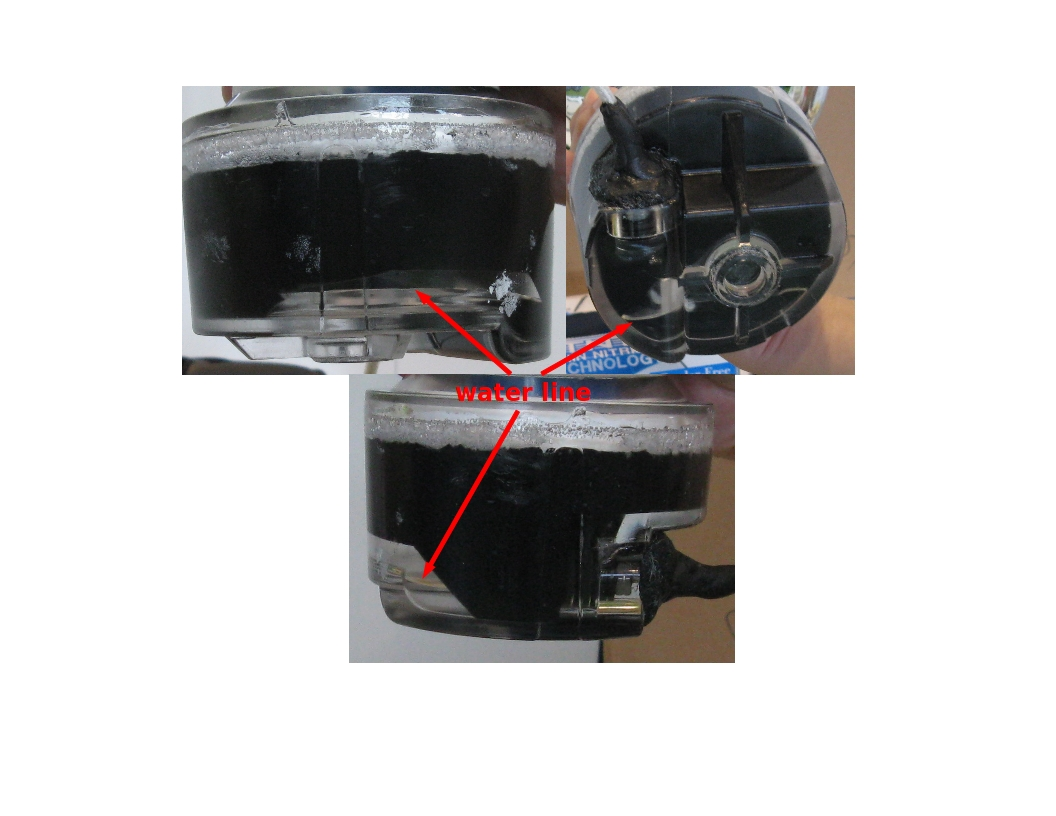
\includegraphics[width=20cm]{PMT7934.jpg}
%}
\end{frame}


\end{document}

